% !TeX program = pdflatex
\documentclass[11pt,a4paper]{article}
\usepackage[utf8]{inputenc}
\usepackage[T1]{fontenc}
\usepackage[turkish]{babel}
\usepackage{lmodern}
\usepackage{geometry}
\usepackage{graphicx}
\usepackage{float}
\usepackage{placeins}
\usepackage{caption}
\usepackage{subcaption}
\usepackage{booktabs}
\usepackage{siunitx}
\usepackage{hyperref}
\usepackage{longtable}
\usepackage{xcolor}
\geometry{margin=2.5cm}
\hypersetup{colorlinks=true,linkcolor=blue,citecolor=blue,urlcolor=blue}
\graphicspath{{../results/}}
% Varsayılan olarak görselleri metin genişliğine sığdır
\setkeys{Gin}{width=0.9\linewidth, keepaspectratio}

\title{NPM Ekosisteminde Yönlü Karmaşık Ağ Analizi}
\author{\textbf{Yusuf Talha ARABACI}}
\date{\today}

\begin{document}
\maketitle

\begin{abstract}
Bu çalışma, NPM ekosistemindeki popüler Top~N paketi, bağımlılık ilişkilerine göre yönlü bir karmaşık ağ (Dependent~$\to$~Dependency) olarak modellemekte ve yapısal riskleri merkeziyet metrikleriyle incelemektedir. Veri, her çalıştırmada API'lerden (öncelikle ecosyste.ms; yedek olarak npm registry ve npms.io) çekilmektedir. Ağ, NetworkX ile kurulmakta; in-degree, out-degree ve betweenness merkeziyet metrikleri hesaplanmaktadır. Büyük graflarda betweenness hesabı örnekleme ($k$) ile hızlandırılmaktadır. Çalışma ayrıca bileşik bir risk skoru (normalize edilmiş in/out/between ağırlıklı toplamı) ve risk tabanlı sağlamlık (robustluk) analizi (kritik düğümlerin çıkarılması) önermektedir. Üretilen tüm çıktılar (CSV/JSON ve PNG/SVG görseller) \texttt{results/} dizininde saklanır.
\end{abstract}

\clearpage

\section{Giriş}
Yazılım tedarik zinciri saldırılarında (SSCA), tek bir bağımlılığın ele geçirilmesi geniş çapta zincirleme etkilere yol açabilir. NPM ekosistemi, yoğun bağımlılık ilişkilerine sahip olup, paketlerin yapısal konumuna göre sistemik risk taşıyabilmektedir. Bu çalışma, Top~N paket üzerinden inşa edilen yönlü bağımlılık ağı ile aşağıdaki sorulara odaklanır:
\begin{itemize}
  \item Hangi düğümler (paketler) yapısal olarak kritik (yüksek in-degree, yüksek betweenness)?
  \item Hangi düğümler geniş bağımlılık yüzeyine sahip (yüksek out-degree)?
  \item Merkeziyetlere dayalı bileşik bir risk skoru ile risk liderleri nasıl sıralanır?
  \item Kritik düğümler çıkarıldığında ağın bağlanırlılığı nasıl değişir (robustluk)?
\end{itemize}

\section{Amaç}
Amaç, yazılım tedarik zinciri güvenliğini paket-içi zafiyetlerin ötesine taşıyarak, bağımlılık ağı topolojisini de hesaba katan yapısal bir ölçüt geliştirmektir. NPM paketleri yönlü bir karmaşık ağ olarak modellenerek, her paketin ağ içindeki yapısal önemi, ele geçirilmesi durumunda yaratabileceği basamaklanma (cascading) etkisi ve bunun sistemik risk üzerindeki nicel etkileri ölçülebilir.

\section{Veri ve Yöntem}
Top~N paket listesi, her çalıştırmada API'lerden çekilir (öncelik ecosyste.ms; yedek olarak npm registry ve npms.io). Bağımlılıklar, npm registry'de paketlerin en güncel sürümlerinin \texttt{dependencies} alanından alınır; isteğe bağlı \texttt{peerDependencies} de eklenebilir. Yönlü ağ, Dependent~$\to$~Dependency yönüyle kurulur. Büyük graflarda betweenness örneklemeli ($k$) hesaplanır.

\section{Ağ Modeli ve Metrikler}
Model, NetworkX ile kurulmuş bir \texttt{DiGraph} yapısıdır. Temel metrikler: (i) \emph{In-degree:} düğüme gelen kenar sayısı (pakete dayanan paket sayısı); (ii) \emph{Out-degree:} düğümün dış bağımlılık sayısı; (iii) \emph{Betweenness:} en kısa yollardaki aracılık (köprü) rolü.

\section{Bulgular}
Bu bölümde, \texttt{results/} dizinindeki çıktılar kullanılarak görsel ve tablolu özetler sunulmaktadır.

\subsection{Ağ Görselleştirmeleri}
\begin{figure}[h]
  \centering
  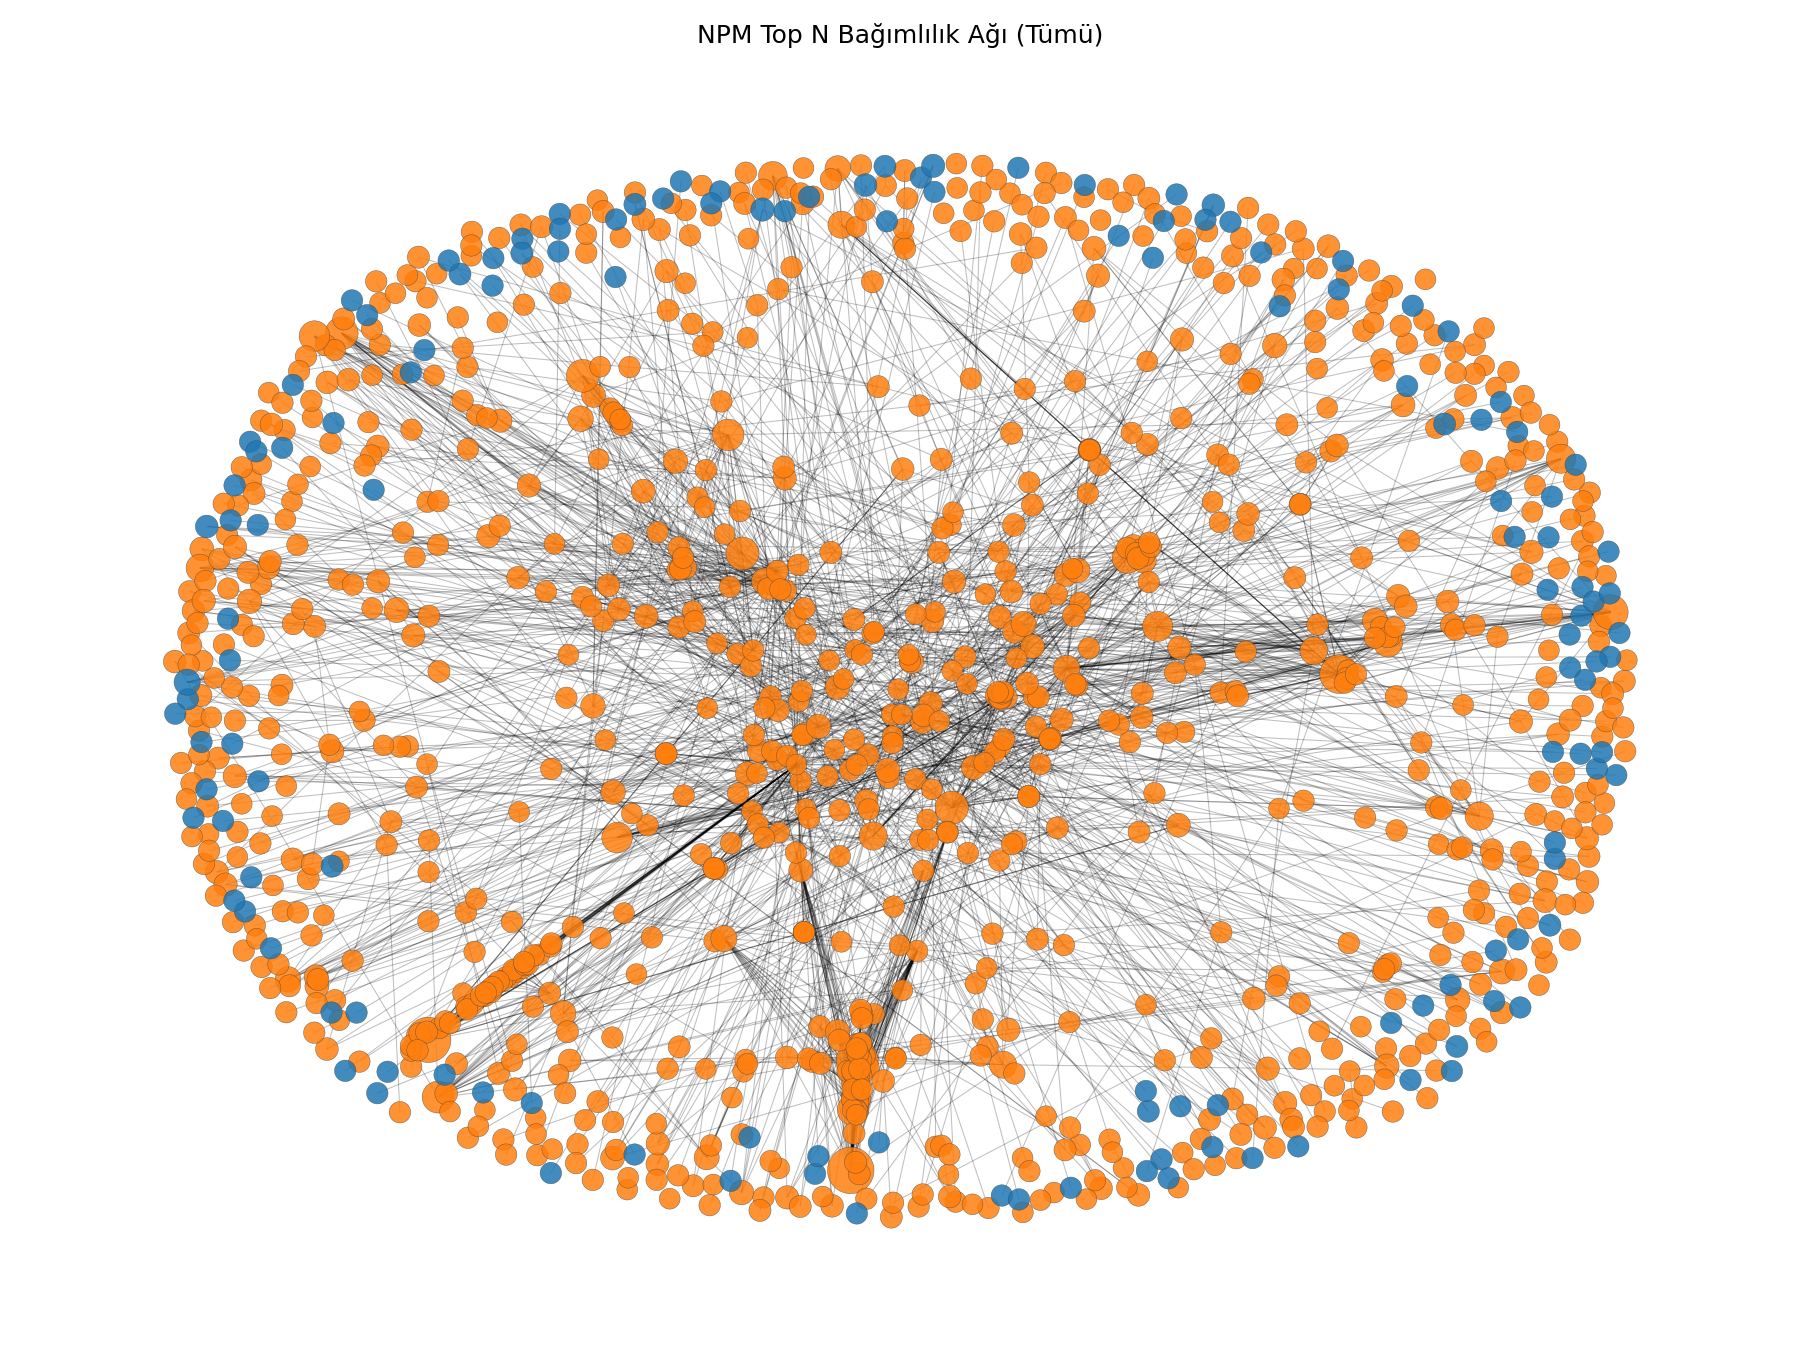
\includegraphics{network_full_topN.png}
  \caption{Top N + bağımlılıkların oluşturduğu yönlü ağ (düğüm boyutu: in-degree; renk: Top N turuncu / diğerleri mavi).}
\end{figure}

\begin{figure}[h]
  \centering
  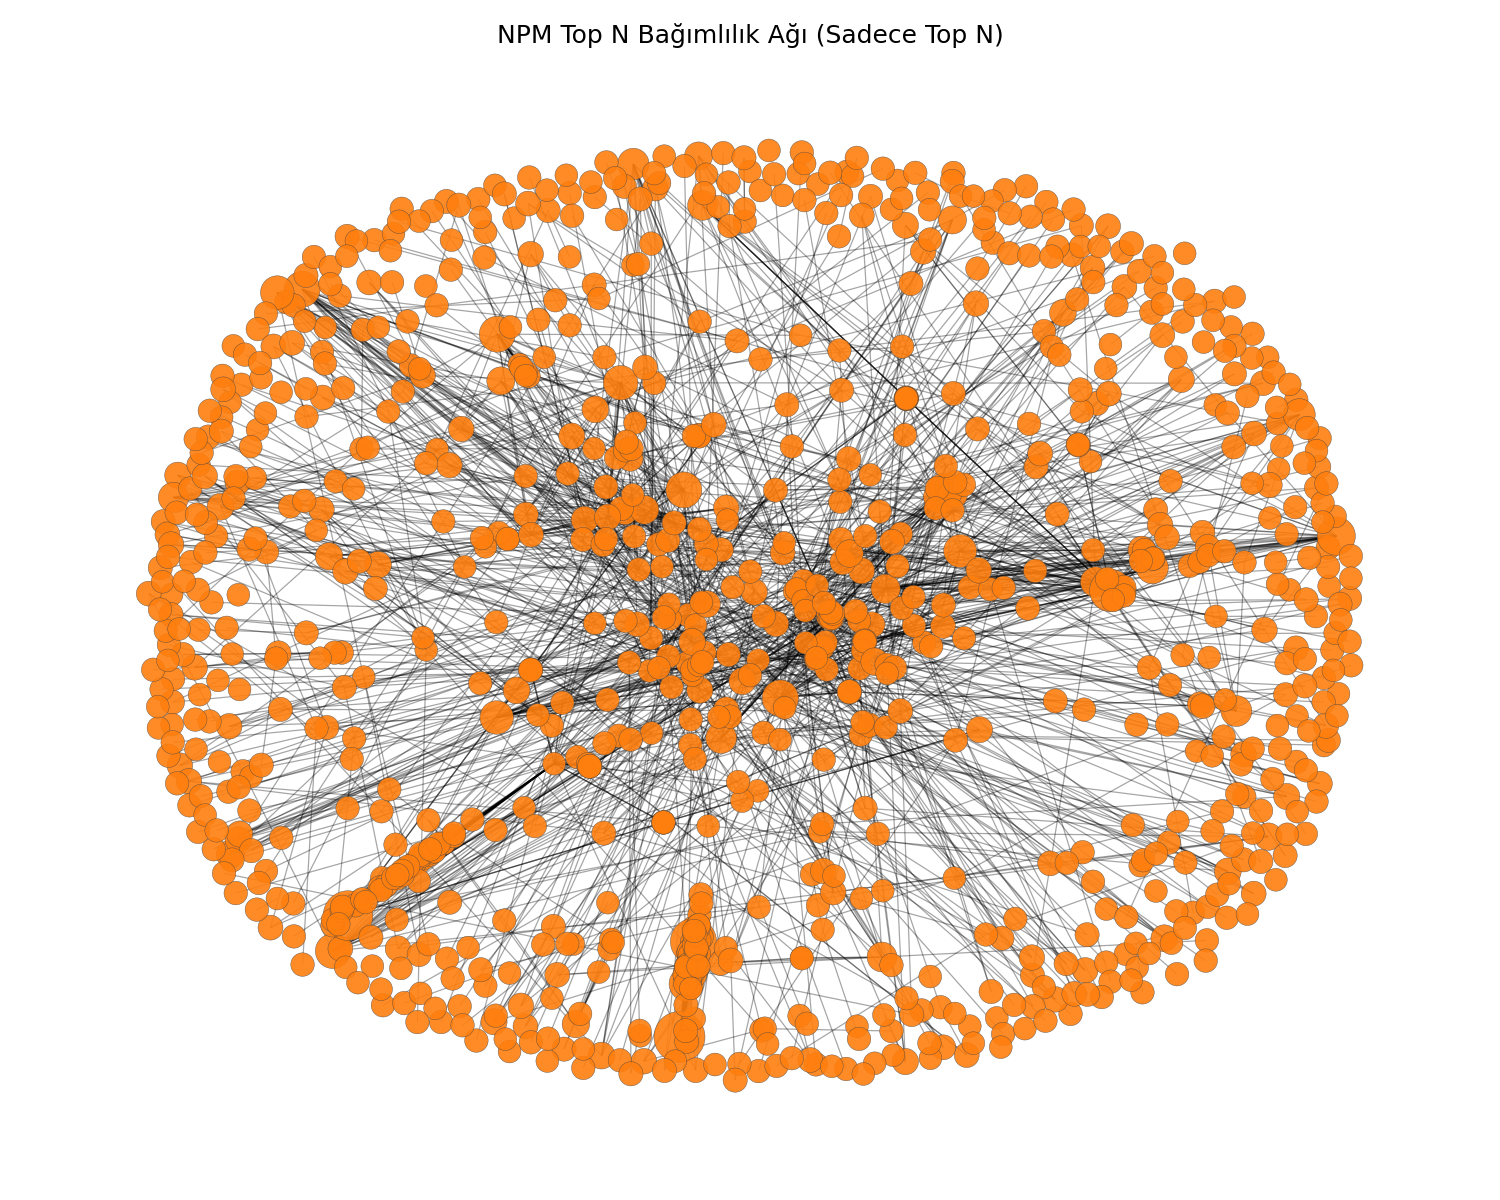
\includegraphics{network_topN_only.png}
  \caption{Sadece Top N düğümlerin indüklenmiş alt-ağı.}
\end{figure}

\subsection{Derece Dağılımları ve Korelasyonlar}
\begin{figure}[h]
  \centering
  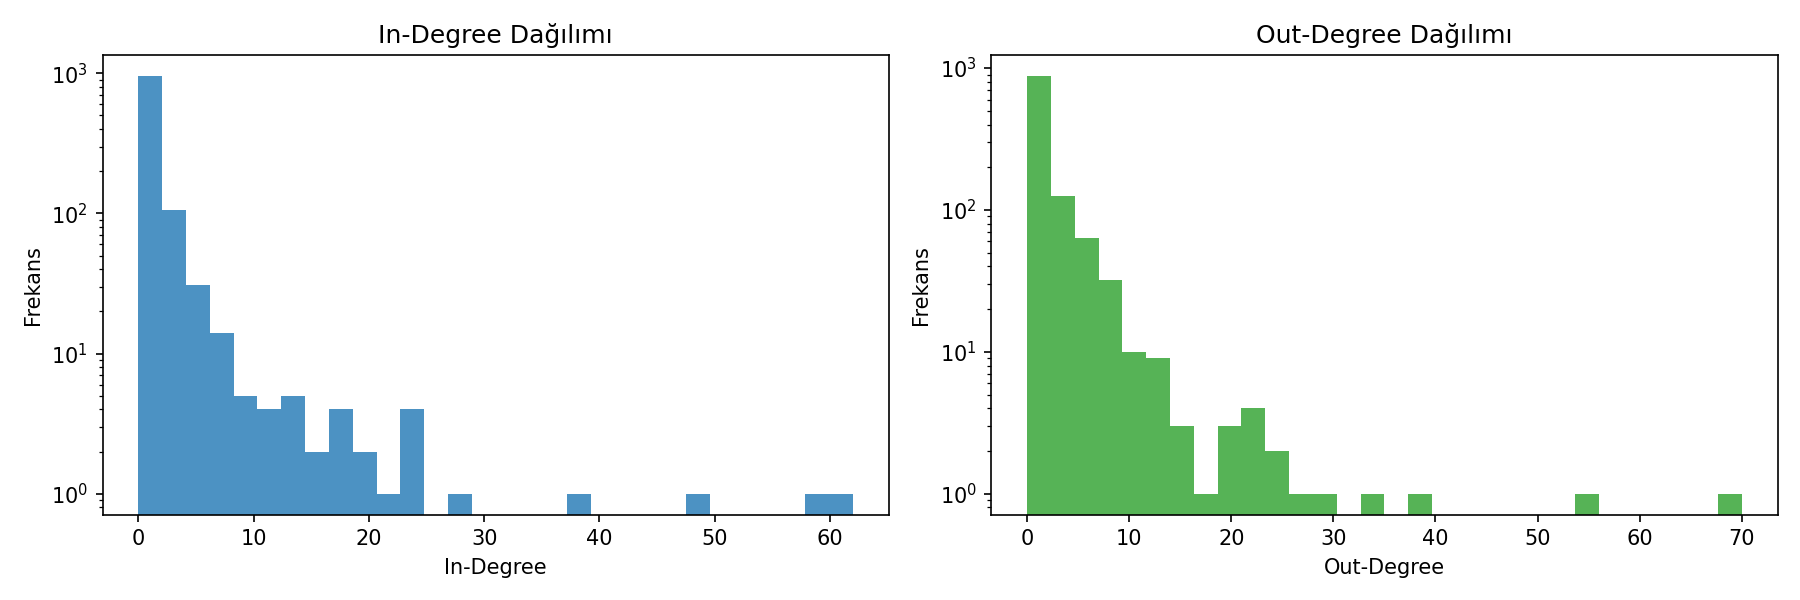
\includegraphics{degree_histograms.png}
  \caption{In-degree ve out-degree histogramları (log ölçek).}
\end{figure}

\begin{figure}[h]
  \centering
  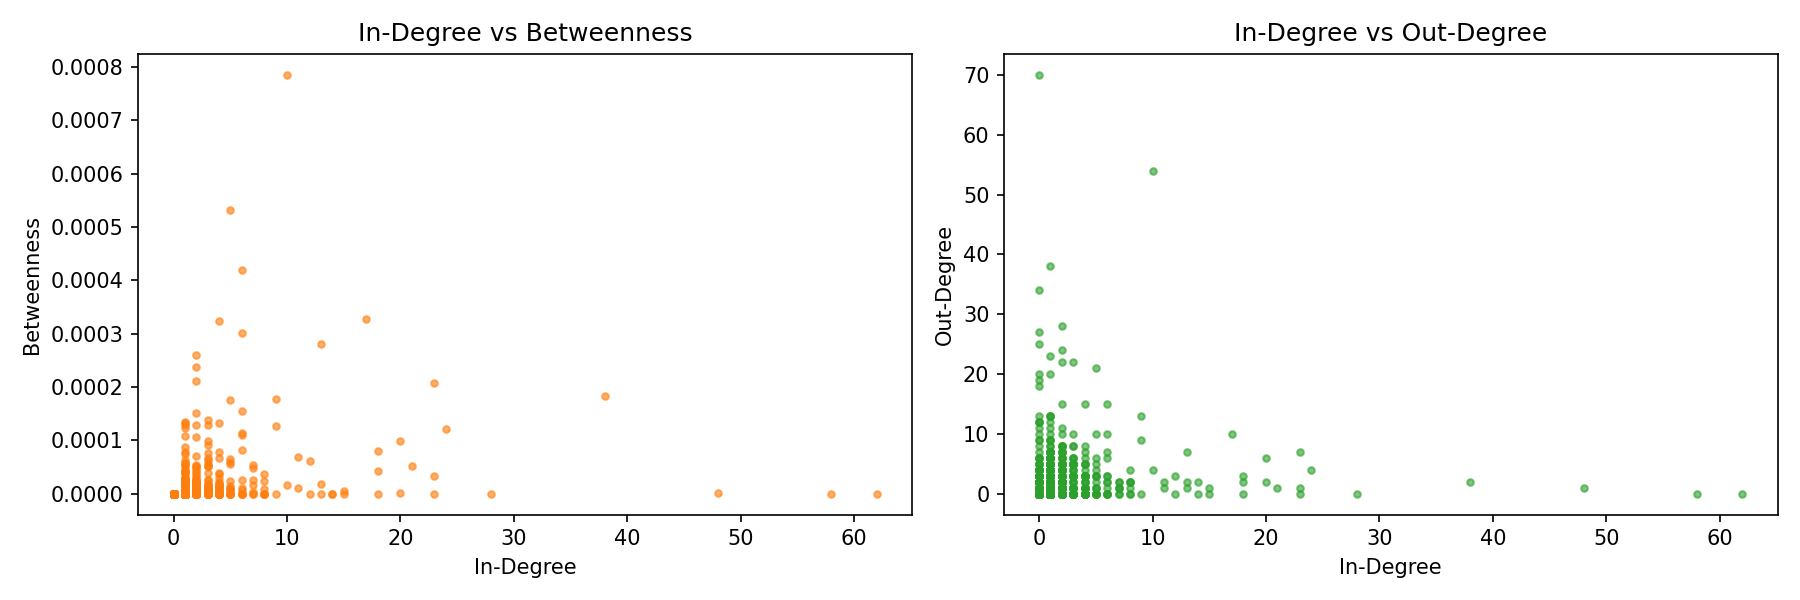
\includegraphics{scatter_correlations.png}
  \caption{Korelasyonlar: In-degree vs Betweenness (solda), In-degree vs Out-degree (sağda).}
\end{figure}

\subsection{Merkeziyet Liderleri}
\begin{figure}[h]
  \centering
  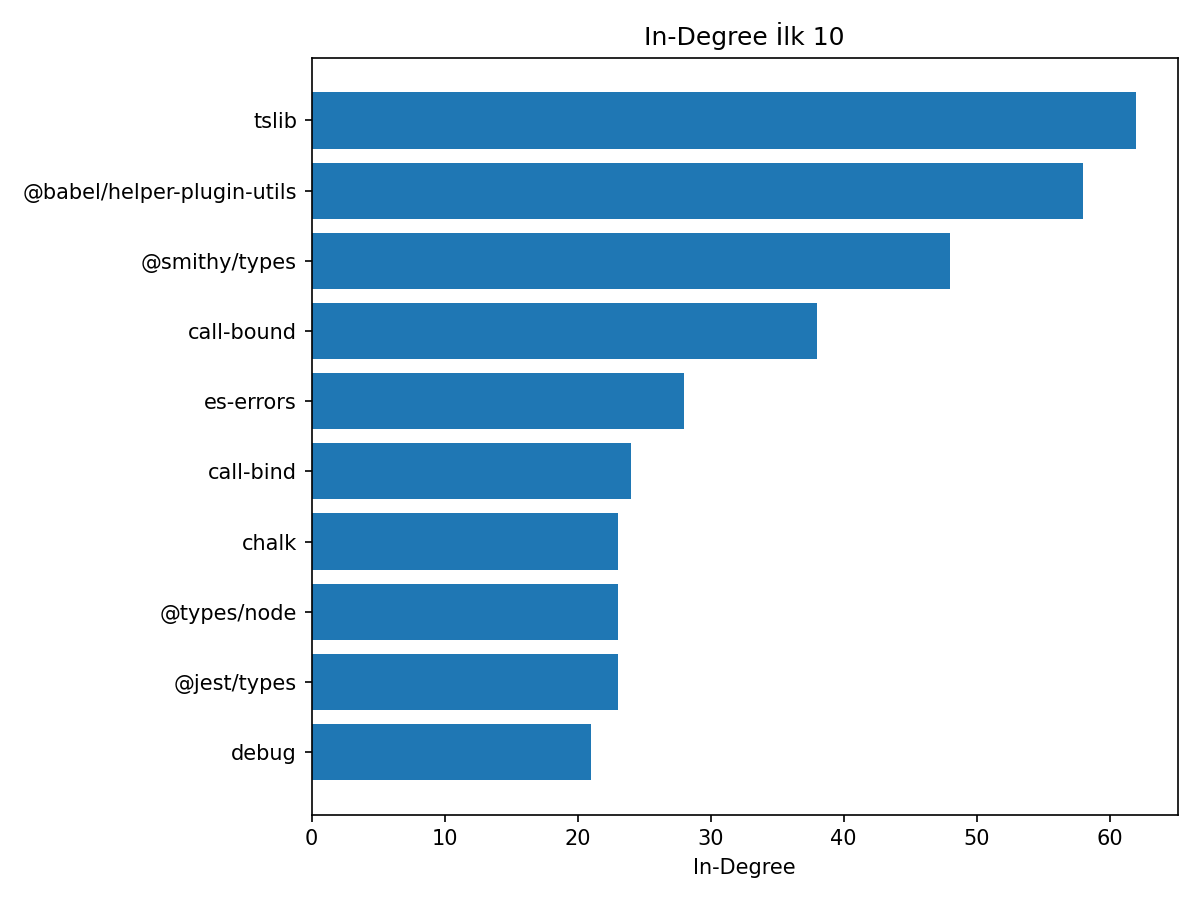
\includegraphics[width=0.48\linewidth]{top10_in_degree.png}
  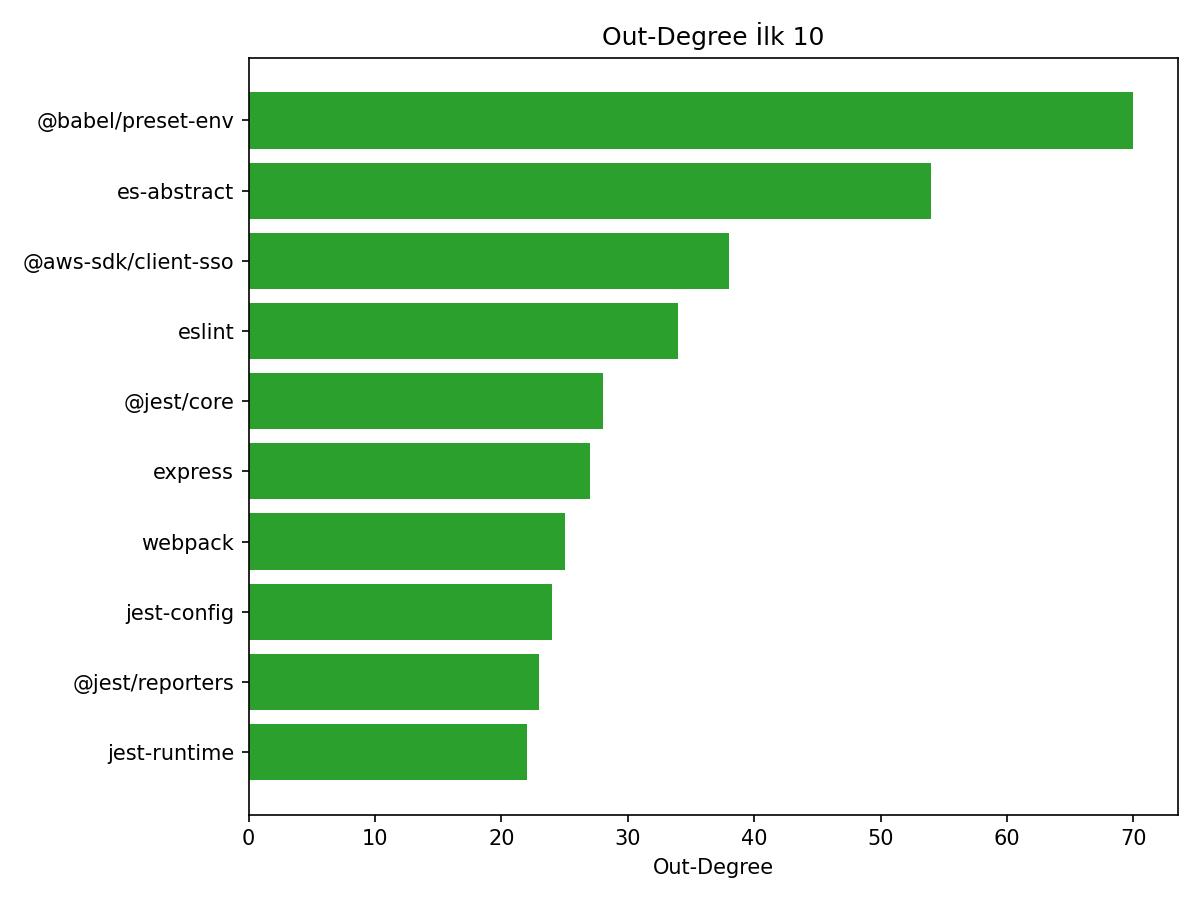
\includegraphics[width=0.48\linewidth]{top10_out_degree.png}
  \caption{İlk 10 In-degree (sol) ve Out-degree (sağ).}
\end{figure}

\begin{figure}[h]
  \centering
  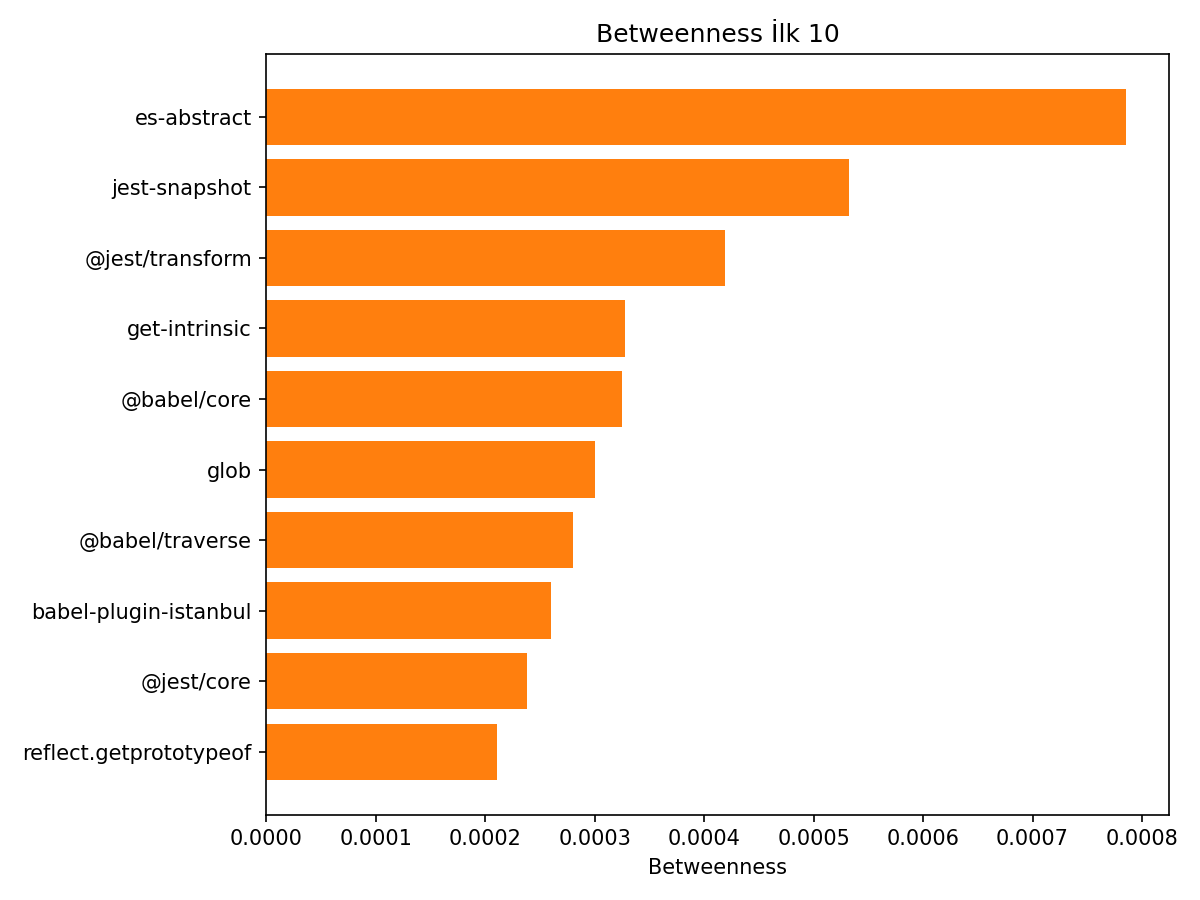
\includegraphics{top10_betweenness.png}
  \caption{İlk 10 Betweenness.}
\end{figure}

\subsection{Risk Skoru ve Robustluk}
\begin{figure}[H]
  \centering
  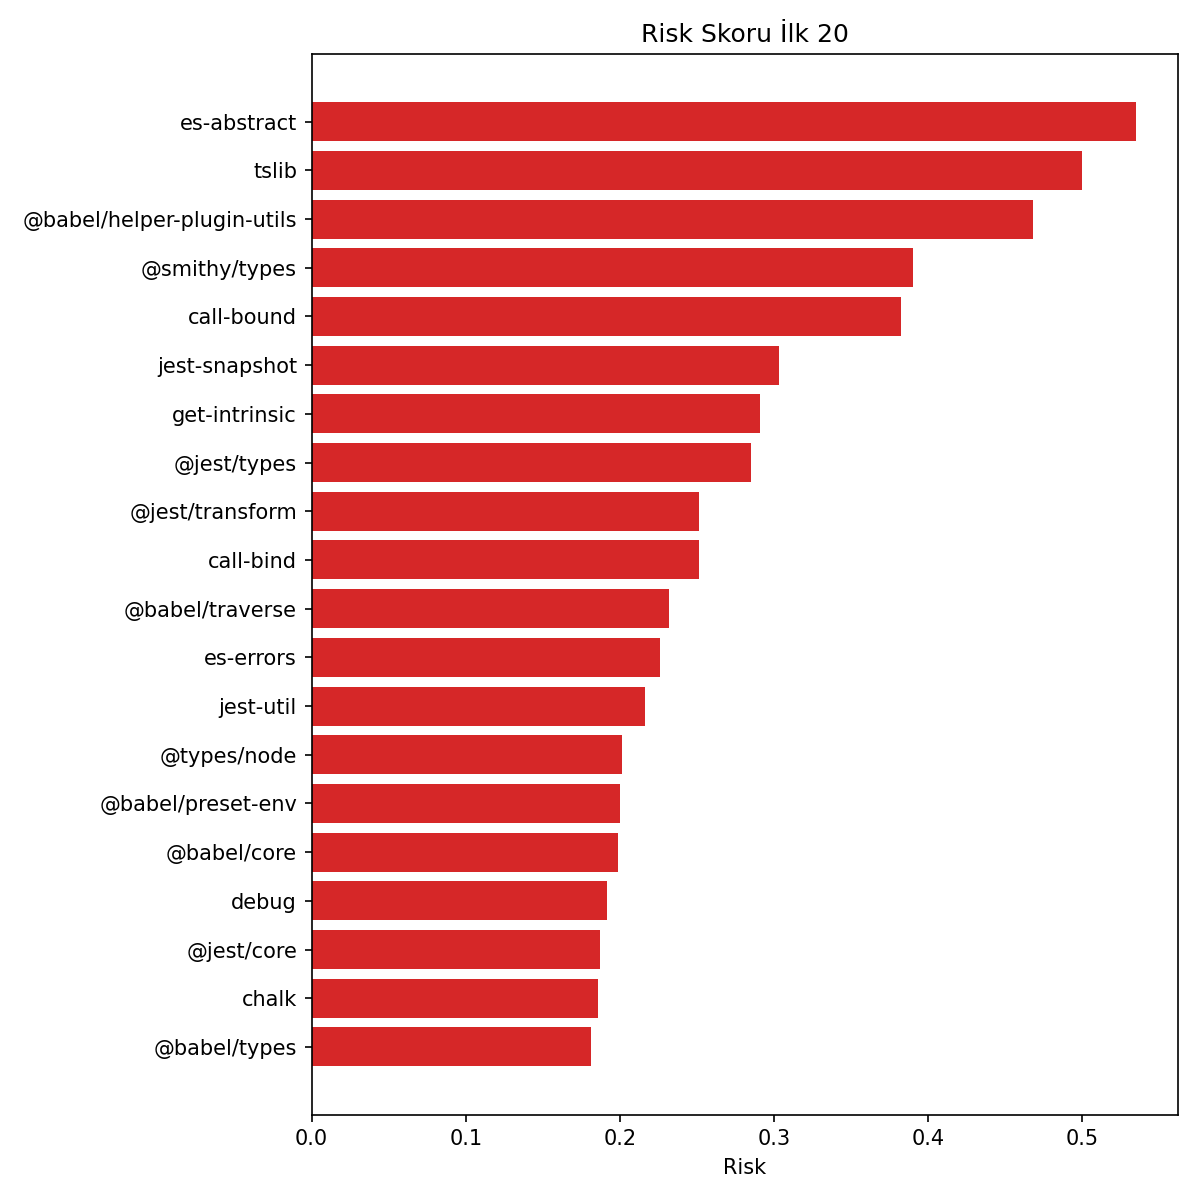
\includegraphics{top20_risk.png}
  \caption{Bileşik risk skoru ile en riskli 20 paket.}
\end{figure}
\FloatBarrier

\paragraph{Kenar Betweenness İlk 10.} Aşağıdaki tablo, en yüksek \emph{edge betweenness} değerine sahip 10 kenarı gösterir.
\IfFileExists{../results/edge_betweenness_top10.tex}{\begin{longtable}{l l r}
\caption{Edge Betweenness Ilk 10 (Yuksek kopru kenarlar)}\\
\toprule
U & V & Edge Betweenness \\
\midrule
\endfirsthead
\toprule
U & V & Edge Betweenness \\
\midrule
\endhead
\bottomrule
\endfoot
\bottomrule
\endlastfoot
@jest/transform & babel-plugin-istanbul & 0.000222 \\
@jest/expect & jest-snapshot & 0.000212 \\
jest-snapshot & @jest/transform & 0.000206 \\
jest & @jest/core & 0.000150 \\
call-bound & get-intrinsic & 0.000150 \\
glob & jackspeak & 0.000147 \\
reflect.getprototypeof & which-builtin-type & 0.000146 \\
jackspeak & @isaacs/cliui & 0.000140 \\
babel-plugin-istanbul & test-exclude & 0.000139 \\
@babel/core & @babel/helper-compilation-targets & 0.000138 \\
\end{longtable}
}{\fbox{edge\_betweenness\_top10.tex bulunamadı}}

\paragraph{Risk Skoru İlk 20.} Bileşik risk skoruna göre ilk 20 paket.
\IfFileExists{../results/risk_scores_top20.tex}{\begin{longtable}{lrrrrr}
\caption{Top 20 Risk Skoru}\\
\toprule
Paket & Risk & In-Degree & Out-Degree & Betweenness & TopN? \\
\midrule
\endfirsthead
\toprule
Paket & Risk & In-Degree & Out-Degree & Betweenness & TopN? \\
\midrule
\endhead
\bottomrule
\endfoot
\bottomrule
\endlastfoot
es-abstract & 0.534931 & 10 & 54 & 0.000785 & True \\
tslib & 0.500000 & 62 & 0 & 0.000000 & True \\
@babel/helper-plugin-utils & 0.467742 & 58 & 0 & 0.000000 & True \\
@smithy/types & 0.390249 & 48 & 1 & 0.000001 & True \\
call-bound & 0.382129 & 38 & 2 & 0.000183 & True \\
jest-snapshot & 0.303511 & 5 & 21 & 0.000532 & True \\
get-intrinsic & 0.290993 & 17 & 10 & 0.000328 & True \\
@jest/types & 0.284735 & 23 & 7 & 0.000207 & True \\
@jest/transform & 0.251456 & 6 & 15 & 0.000419 & True \\
call-bind & 0.251171 & 24 & 4 & 0.000121 & True \\
@babel/traverse & 0.231984 & 13 & 7 & 0.000280 & True \\
es-errors & 0.225806 & 28 & 0 & 0.000000 & True \\
jest-util & 0.216164 & 20 & 6 & 0.000099 & True \\
@types/node & 0.201331 & 23 & 1 & 0.000034 & True \\
@babel/preset-env & 0.200000 & 0 & 70 & 0.000000 & True \\
@babel/core & 0.199075 & 4 & 15 & 0.000324 & True \\
debug & 0.191845 & 21 & 1 & 0.000051 & True \\
@jest/core & 0.187008 & 2 & 28 & 0.000238 & True \\
chalk & 0.185484 & 23 & 0 & 0.000000 & True \\
@babel/types & 0.181088 & 18 & 2 & 0.000079 & True \\
\end{longtable}
}{\fbox{risk\_scores\_top20.tex bulunamadı}}

\paragraph{Dereceye Göre İlk 20.} In/Out/Betweenness sıralamaları.
\IfFileExists{../results/metrics_top20_in_degree.tex}{\begin{table}[h]
\centering
\\\caption{Top 20 In-Degree (Toplam Düğümler)}
\begin{tabular}{lrrrr}
\toprule
Paket & In-Degree & Out-Degree & Betweenness & TopN? \\ \midrule
tslib & 62 & 0 & 0.000000 & True \\
@babel/helper-plugin-utils & 58 & 0 & 0.000000 & True \\
@smithy/types & 48 & 1 & 0.000001 & True \\
call-bound & 38 & 2 & 0.000183 & True \\
es-errors & 28 & 0 & 0.000000 & True \\
call-bind & 24 & 4 & 0.000121 & True \\
@jest/types & 23 & 7 & 0.000207 & True \\
@types/node & 23 & 1 & 0.000034 & True \\
chalk & 23 & 0 & 0.000000 & True \\
debug & 21 & 1 & 0.000051 & True \\
@aws-sdk/types & 20 & 2 & 0.000002 & True \\
jest-util & 20 & 6 & 0.000099 & True \\
@babel/types & 18 & 2 & 0.000079 & True \\
define-properties & 18 & 3 & 0.000043 & True \\
graceful-fs & 18 & 0 & 0.000000 & True \\
get-intrinsic & 17 & 10 & 0.000328 & True \\
es-object-atoms & 15 & 1 & 0.000006 & True \\
gopd & 15 & 0 & 0.000000 & True \\
@smithy/protocol-http & 14 & 2 & 0.000000 & True \\
semver & 14 & 0 & 0.000000 & True \\
\bottomrule
\end{tabular}
\end{table}
}{\fbox{metrics\_top20\_in\_degree.tex bulunamadı}}
\IfFileExists{../results/metrics_top20_out_degree.tex}{\begin{longtable}{lrrrr}
\caption{Top 20 Out-Degree (Toplam Dugumler)}\\
\toprule
Paket & Out-Degree & In-Degree & Betweenness & TopN? \\
\midrule
\endfirsthead
\toprule
Paket & Out-Degree & In-Degree & Betweenness & TopN? \\
\midrule
\endhead
\bottomrule
\endfoot
\bottomrule
\endlastfoot
@babel/preset-env & 70 & 0 & 0.000000 & True \\
es-abstract & 54 & 10 & 0.000785 & True \\
@aws-sdk/client-sso & 38 & 1 & 0.000075 & True \\
eslint & 34 & 0 & 0.000000 & True \\
@jest/core & 28 & 2 & 0.000238 & True \\
express & 27 & 0 & 0.000000 & True \\
webpack & 25 & 0 & 0.000000 & True \\
jest-config & 24 & 2 & 0.000128 & True \\
@jest/reporters & 23 & 1 & 0.000039 & True \\
jest-runner & 22 & 2 & 0.000042 & True \\
jest-runtime & 22 & 3 & 0.000129 & True \\
jest-snapshot & 21 & 5 & 0.000532 & True \\
jest-circus & 20 & 1 & 0.000040 & True \\
jsdom & 20 & 0 & 0.000000 & True \\
eslint-plugin-import & 19 & 0 & 0.000000 & True \\
eslint-plugin-react & 18 & 0 & 0.000000 & True \\
@babel/core & 15 & 4 & 0.000324 & True \\
@jest/transform & 15 & 6 & 0.000419 & True \\
babel-preset-current-node-syntax & 15 & 2 & 0.000151 & True \\
@aws-sdk/core & 13 & 9 & 0.000127 & True \\
\end{longtable}
}{\fbox{metrics\_top20\_out\_degree.tex bulunamadı}}
\IfFileExists{../results/metrics_top20_betweenness.tex}{\begin{table}[h]
\centering
\caption{Top 20 Betweenness (Toplam D\"ug\"umler)}
\begin{tabular}{lrrrr}
\toprule
Paket & Betweenness & In-Degree & Out-Degree & TopN? \\ \midrule
es-abstract & 0.000785 & 10 & 54 & True \
jest-snapshot & 0.000532 & 5 & 21 & True \
@jest/transform & 0.000419 & 6 & 15 & True \
get-intrinsic & 0.000328 & 17 & 10 & True \
@babel/core & 0.000324 & 4 & 15 & True \
glob & 0.000301 & 6 & 6 & True \
@babel/traverse & 0.000280 & 13 & 7 & True \
babel-plugin-istanbul & 0.000260 & 2 & 5 & True \
@jest/core & 0.000238 & 2 & 28 & True \
reflect.getprototypeof & 0.000211 & 2 & 8 & True \
@jest/types & 0.000207 & 23 & 7 & True \
call-bound & 0.000183 & 38 & 2 & True \
jest-message-util & 0.000178 & 9 & 9 & True \
@babel/helper-compilation-targets & 0.000176 & 5 & 5 & True \
jest-haste-map & 0.000156 & 6 & 10 & True \
babel-preset-current-node-syntax & 0.000151 & 2 & 15 & True \
@babel/generator & 0.000139 & 3 & 5 & True \
which-builtin-type & 0.000134 & 1 & 13 & True \
browserslist & 0.000133 & 4 & 5 & True \
jackspeak & 0.000132 & 1 & 1 & True \
\bottomrule
\end{tabular}
\end{table}
}{\fbox{metrics\_top20\_betweenness.tex bulunamadı}}

\begin{figure}[h]
  \centering
  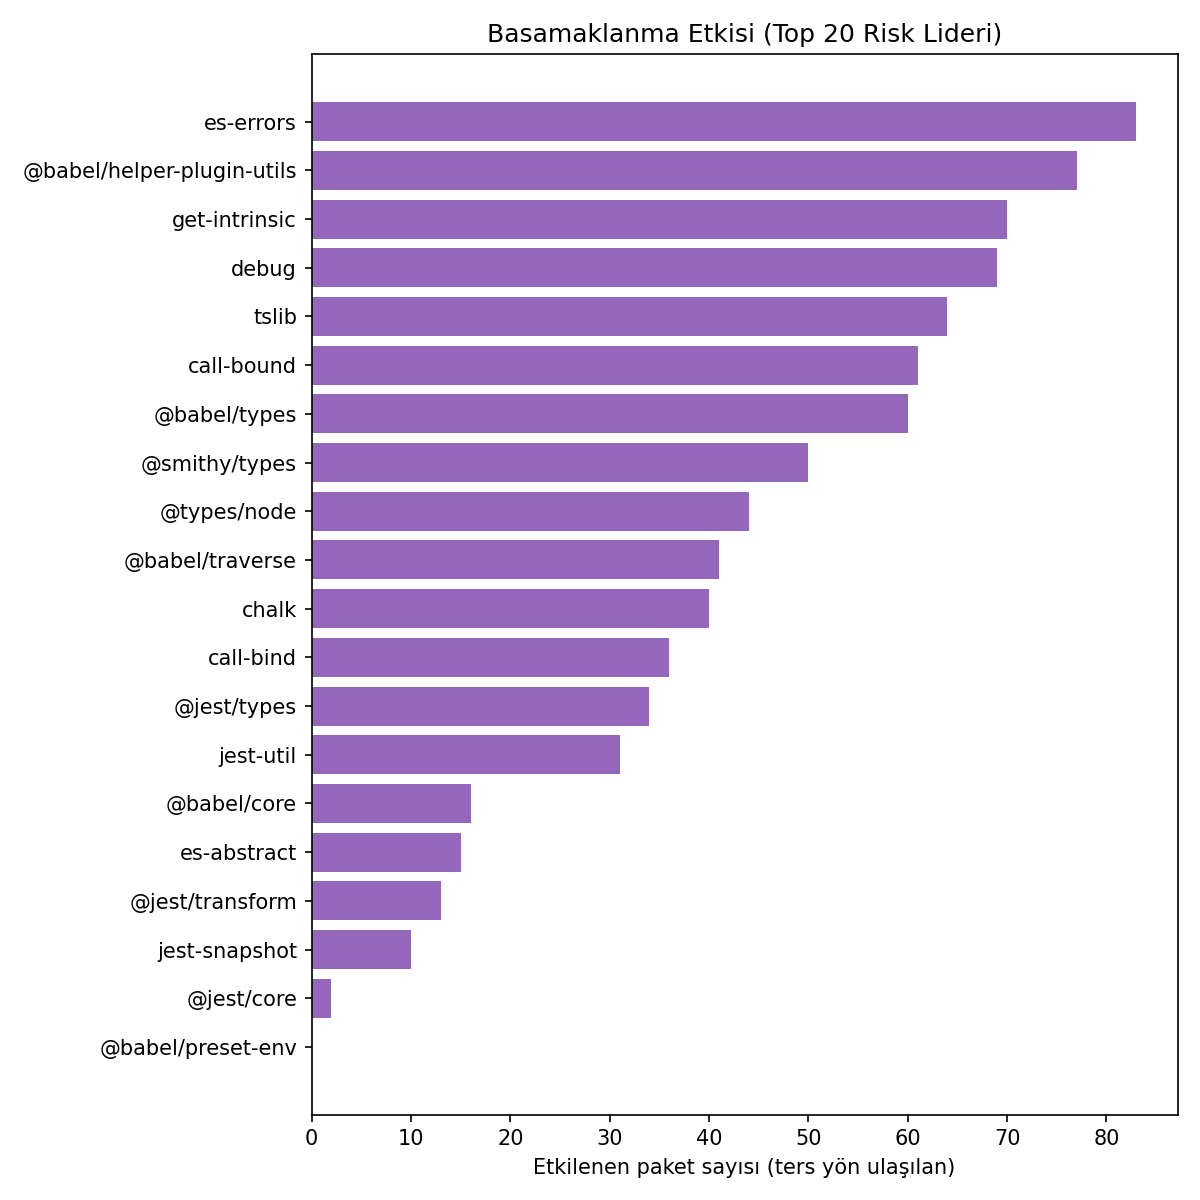
\includegraphics[width=0.75\textwidth]{cascade_impact_top20.png}
  \caption{Risk skoruna göre en riskli 20 paket için basamaklanma (cascading impact) büyüklüğü.}
\end{figure}
\IfFileExists{../results/cascade_impact_top20.tex}{\begin{table}[h]
\centering
\caption{Basamaklanma Etkisi: Top 20 (Ters y"onde etkilenebilecek paket say\i s\i)}
\begin{tabular}{l r}
\toprule
Paket & Etkilenen Paket Say\i s\i \\ \midrule
es-errors & 83 \
@babel/helper-plugin-utils & 77 \
get-intrinsic & 70 \
debug & 69 \
tslib & 64 \
call-bound & 61 \
@babel/types & 60 \
@smithy/types & 50 \
@types/node & 44 \
@babel/traverse & 41 \
chalk & 40 \
call-bind & 36 \
@jest/types & 34 \
jest-util & 31 \
@babel/core & 16 \
es-abstract & 15 \
@jest/transform & 13 \
jest-snapshot & 10 \
@jest/core & 2 \
@babel/preset-env & 0 \
\bottomrule
\end{tabular}
\end{table}
}{\fbox{cascade\_impact\_top20.tex bulunamadı}}

\paragraph{Risk--Basamaklanma İlişkisi.} Ek olarak, risk skoru ile basamaklanma etkisi arasındaki ilişki incelenmiştir.
\begin{figure}[h]
  \centering
  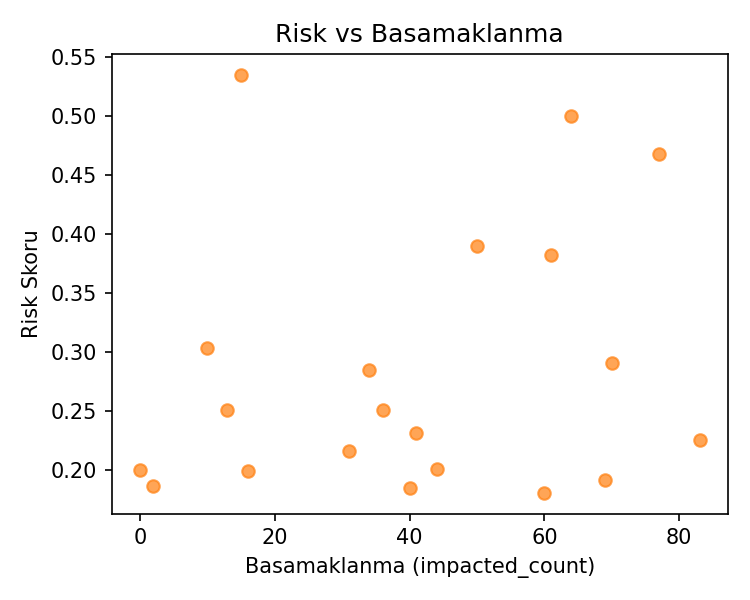
\includegraphics[width=0.6\textwidth]{risk_vs_cascade.png}
  \caption{Risk skoru ile basamaklanma etkisi arasındaki ilişki (scatter).}
\end{figure}

\section{Öne Çıkan Paketler (Kısa Açıklamalar)}
Aşağıda, ağda yapısal olarak öne çıkan ve sık karşılaşılan 20 paket için kısa açıklamalar verilmiştir. Liste, geniş kullanım alanları nedeniyle tedarik zinciri riskine işaret eden altyapı kütüphanelerini vurgular.
\begin{enumerate}
  \item \texttt{es-abstract}: ECMAScript spesifikasyonundaki soyut işlemleri uygular; çok sayıda paketin altyapısında kullanılır.
  \item \texttt{tslib}: TypeScript derleyicisinin çalışma zamanı yardımcılarını içerir; yaygın kullanımı nedeniyle kritik olabilir.
  \item \texttt{@babel/helper-plugin-utils}: Babel eklentileri geliştirmek için yardımcı fonksiyonlar sağlar; ekosistemde geniş bağımlılık ağına sahiptir.
  \item \texttt{@smithy/types}: AWS SDK (v3) içindeki tip altyapısı; büyük ölçekli projelerde zincir etkisine adaydır.
  \item \texttt{call-bound}: JS \emph{intrinsic} metotları güvenli biçimde çağırmak/bağlamak için yardımcı; çok sayıda modül tarafından kullanılır.
  \item \texttt{jest-snapshot}: Jest için \emph{snapshot} testleri; test zincirinde kritik, dolaylı etkisi olabilir.
  \item \texttt{get-intrinsic}: ECMAScript \emph{intrinsic} nesnelerini güvenli elde etmek için yardımcı; alt katmanda yaygın kullanılır.
  \item \texttt{@jest/types}: Jest ekosisteminde ortak tip altyapısı; modüller arası etkileşimi artırır.
  \item \texttt{@jest/transform}: Jest'te kaynak dönüşüm (transpile) katmanı; test-üretim zincirinde önemli.
  \item \texttt{call-bind}: Fonksiyon bağlaması için yardımcı; ağda düğüm yoğunluğu yüksek küçük kütüphanelerden.
  \item \texttt{@babel/traverse}: AST üzerinde gezinme; kod dönüşüm süreçlerinde temel modüllerden.
  \item \texttt{es-errors}: ECMAScript hata tipleri ve soyut işlemler için yardımcı; altyapı rolünde.
  \item \texttt{jest-util}: Jest ekosisteminde çeşitli yardımcılar; test altyapısında kritik rol.
  \item \texttt{@types/node}: Node.js için tip deklarasyonları; TypeScript ile yaygın standart bağımlılık.
  \item \texttt{@babel/preset-env}: Hedef ortama göre derleme yapan Babel preset'i; yüksek yayılım riski.
  \item \texttt{@babel/core}: Babel'in çekirdeği; derleme zincirinin üst katmanı, sistemik risk yüksektir.
  \item \texttt{debug}: \emph{Namespace}'li loglama; geçmişte tedarik zinciri saldırısı vakaları olmuştur.
  \item \texttt{chalk}: Terminal stil kütüphanesi; popülerlik nedeniyle hedef olabilen modüllerden.
  \item \texttt{@jest/core}: Jest'in çekirdeği; test sürecinin kalbinde.
  \item \texttt{@babel/types}: AST düğümlerini oluşturma/denetleme; kod dönüşümünde temel işlevler.
\end{enumerate}

\section{Risk Skoru Tanımı}
Normalize edilmiş metrikler (min--max) üzerinden ağırlıklandırılmış bir risk skoru tanımlanmıştır: $\mathrm{risk}(n) = w_{in} \, \tilde d_{in}(n) + w_{out} \, \tilde d_{out}(n) + w_b \, \tilde b(n)$. Ağırlıklar (örn. $w_{in}=0.5,\ w_{out}=0.2,\ w_b=0.3$) senaryoya göre ayarlanabilir.

\section{Robustluk Analizi}
Risk skoruna göre en kritik $k\in\{1,3,5\}$ düğüm çıkarıldığında zayıf bağlanırlık bileşen sayısı, en büyük bileşen boyutu ve (mümkünse) çap raporlanır (bkz. \texttt{robustness\_risk.json}).

\section{Sınırlamalar}
\textbf{Sınırlamalar:} (i) Varsayılan olarak yalnızca \texttt{dependencies} kullanılır; \texttt{peerDependencies} isteğe bağlıdır. (ii) Betweenness hesabı büyük graflarda örneklemelidir; kesin değerlerin yakınsaması ağ büyüklüğüne ve $k$ seçimine bağlıdır. (iii) Global \emph{dependent} sayıları doğrudan dahil edilmemiştir.

\section{Sonuç}
Bu çalışma, NPM ekosistemindeki popüler paketler için yönlü bağımlılık ağını kullanarak yapısal riskleri nicel olarak analiz etmektedir. Merkeziyet metrikleri, bileşik risk skoru ve robustluk analizleri, kritik düğümlerin ve köprülerin pratikte nasıl belirleneceğine dair bir çerçeve sunar.

\paragraph{Çoğaltılabilirlik.} Tüm kod ve çıktı üretimi depo içindedir. \texttt{analysis.ipynb} defteri çalıştırılarak \texttt{results/} dizini yeniden üretilebilir ve bu makale \LaTeX~dosyası ile raporlanabilir.

\bibliographystyle{plain}
\begin{thebibliography}{9}
\bibitem{newman2010} Newman, M. (2010). \emph{Networks: An Introduction}. Oxford University Press.
\bibitem{brandes2001} Brandes, U. (2001). A faster algorithm for betweenness centrality. \emph{Journal of Mathematical Sociology}.
\bibitem{barabasi2016} Barab\'asi, A.-L. (2016). \emph{Network Science}. Cambridge University Press.
\end{thebibliography}

\end{document}

